\documentclass{simcenterdocumentation}
\usepackage[backend=biber]{biblatex}
\usepackage{subfig}
\usepackage{multirow}
\usepackage{adjustbox} % to adjust table width
\usepackage{graphicx} %Loading the package
\usepackage{longtable}
\usepackage{cleveref}
\graphicspath{{../Common/}{.}} %Setting the graphicspath
\makeatletter % Search additional directories for inputs
\def\input@path{{../Common/}{.}}
%or: \def\input@path{{/path/to/folder/}{/path/to/other/folder/}}
\makeatother

%% Add unicode support for special characters
%%\usepackage[utf8x]{inputenc}

% To compile this file, run "latex/pdflatex codedoc", then "biber codedoc"b
% (or "bibtex codedoc", if the output from latex asks for that instead),
% and then "latex/pdflatex codedoc" (without the quotes in each case).

% Double spacing, if you want it.  Do not use for the final copy. Can also specify
% draft as a document class option. This will generate double spacing and placeholders
% for title page and header images
%% \def\dsp{\def\baselinestretch{2.0}\large\normalsize}
%% \dsp

\bibliography{references}

\begin{document}
% Declarations for Front Matter
% Software title followed by optional second line
\title{     {\fontfamily{qhv}\selectfont \textbf{\textit{SWIM}} }       \\ Shear Wall Intelligent Modeling: AI-enabled finite element modeling of concrete shear walls}
% Use superscripts to indicate author affiliations
\author{Chaofeng Wang and Frank McKenna}
\institutions{NHERI SimCenter, UC Berkeley}
\softwarename{{\fontfamily{qhv}\selectfont \textit{SWIM}}}
\softwareversion{1.0.1}
\softwarepage{https://github.com/NHERI-SimCenter/SWIM}

%%% DON'T MESS WITH THESE SETTINGS %%%%%%%%%%%%%%%%%%%%%%%%%%%%%%%%
\hypersetup{pageanchor=false}
\maketitle
\copyrightpage
\acknowledgments

\hypersetup{pageanchor=true}
\begin{frontmatter}

\pagestyle{plain}
{
  \renewcommand{\thispagestyle}[1]{}
  \tableofcontents
  \clearpage
  \listoffigures
  \clearpage
  \listoftables
}

\end{frontmatter}
\pagestyle{somewhatsimple}
%%%%%%%%%%%%%%%%%%%%%%%%%%%%%%%%%%%%%%%%%%%%%%%%%%%%%%%%%%%%%%%%%%%
% Create separate tex files for each chapter and provide them as inputs

\chapter{About}
\label{chap:about}
The intended audience for the \texttt{\getsoftwarename{}} Application (\texttt{\getsoftwarename{}} App) is educators, researchers and practitioners
interested in performing finite element modeling of cyclic shear experiments of concrete shear walls. \texttt{\getsoftwarename{}}  is the acronym of shear wall intelligent modeling. 
The word ``intelligent" indicates this app is integrated with machine learning algorithms assisting users in the modeling.   \\



Given that the properties of the concrete shear wall and the loading events are known,
 \texttt{\getsoftwarename{}} provides nonlinear material models for simulating the wall behavior under cyclic loading.\\

This is an open-source research application. The source code can be found on: 
 \href{https://github.com/NHERI-SimCenter/SWIM}{\texttt{\getsoftwarename{}}
Github page}.\\


This is Version \getsoftwareversion{} of the tool. Users are
encouraged to comment on what additional features and capabilities
they would like to see in this application. These requests and
feedback can be submitted through an anonymous \insertsurveylink{user
survey}; we greatly appreciate any input you have. If there are
features you want, chances are many of your colleagues also would
benefit from them. 


\chapter{Installation Instructions}
\label{chap:installation}
All SimCenter applications are available at
the \href{https://simcenter.designsafe-ci.org/research-tools/overview/}{SimCenter
website} under \emph{Research Tools} or \emph{Learning Tools}. The following sections outline
the steps necessary to download and install the \texttt{\getsoftwarename{}}
application. The SimCenter applications do require that you install a
number of other applications that are needed to run the workflows on
your local machine as well as at DesignSafe. \\


%===============================================================================
\section{Download the Application}
%===============================================================================

% \subsection{Download the Application Files}

To download the \texttt{\getsoftwarename{}} application navigate to
the \getsoftwarepage{\texttt{\getsoftwarename{}} page} and click on
the \emph{Download App \& User Manual} link on the right side of the
page. This will bring you to another page which contains a list of downloadable files and directories.


There are at least four files available for download from this page: 
\begin{enumerate}
    \item The PDF file is the User Manual that you are reading now.
    \item The MOV file is an video that provides an introduction to the usage of the application.
    \item The ZIP file is an archive that contains the application files for a Windows operating system.
    \item The DMG file is an archive that contains the application files for a Mac OS X operating system.
\end{enumerate}

To download the \texttt{\getsoftwarename{}} application click on the link for
the appropriate file for your operating system and then click on the
Download button at bottom right corner of the ensuing pop-up window to
download it. You need to unpackage the application from the downloaded
file and place it in a location on your filesystem. On Windows, we
recommend that you create a \texttt{C:/SimCenter/\getsoftwarename{}}
directory and extract the contents of the \texttt{ZIP} archive
there. It is also recommended to run the included installer for Visual C/C++ runtime library(vc\_redist.x64.exe). On Mac, we recommend you copy the application to either your
Documents folder or your Desktop folder. You are free to place the
applications anywhere you wish, you will just need to make the
appropriate adjustments with the following instructions if you do so. \\



%===============================================================================
\clearpage
\section{Test the \texttt{\getsoftwarename{}} application}
\label{sec:test_local}


Click on the  icon of  \texttt{\getsoftwarename{}} to open the application.
Click the ``SAM" tab to see the configuration of structural analysis model (\Cref{fig:testing}). 
Input the path of OpenSees executable in to ``FEM engine" at the bottom of the SAM tab.



Click ``Analyze" button at the button of the ``Input" panel to start the finite element analysis.
If the application is running correctly, you'll see a progress bar displayed at the middle of the app, which shows the percentage of steps performed. 
When the FE analysis is done, you'll see it shows a message saying ``Analysis is done."  (\Cref{fig:testing}).
And when you click ``I know.", the progress bar will disappear. Now if the ``Play" button is played, you should be able to see animations at the right side of the application.

\begin{figure}[!htbp]
  \centering {
    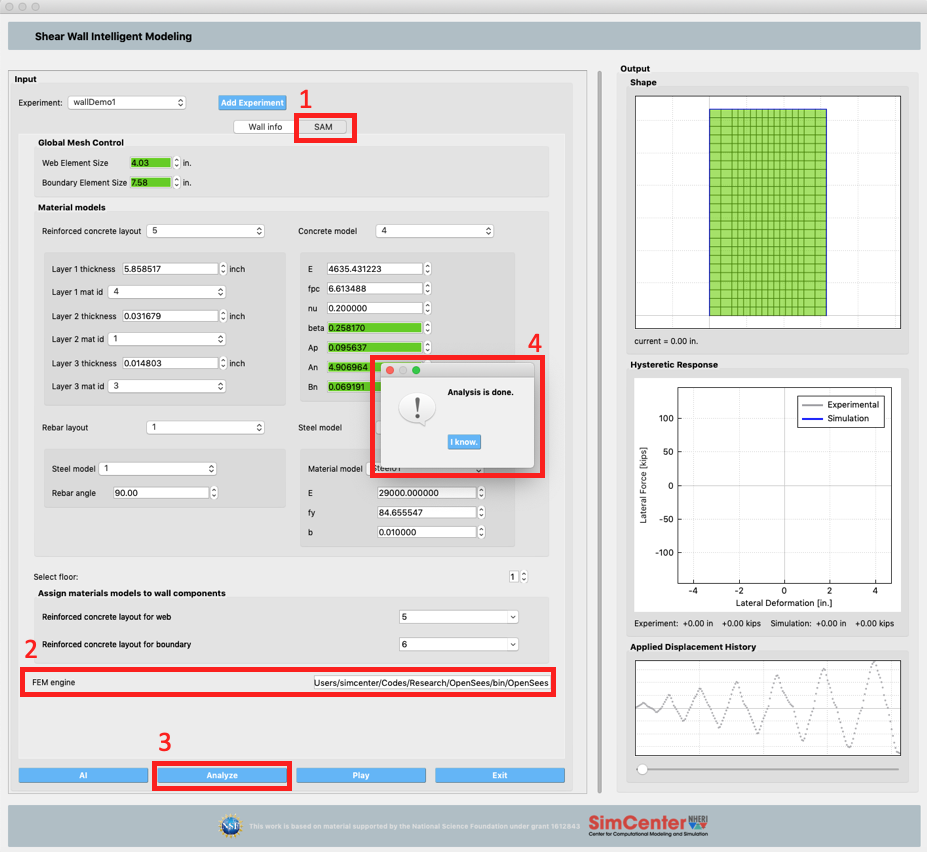
\includegraphics[width=0.6\textwidth]
    {figures/SWIM_analysisisdone-green.png} }
  \caption{Testing SWIM}
  \label{fig:testing}
\end{figure}



%===============================================================================


\chapter{Usage}
\label{chap:usage}
There are two panels in this application.
On the left is the ``Input" panel, where the user can load an experiment, configure the finite element model, and run analysis.
On the right is the ``Output" panel, where the user see results visualized, such as the mesh of the wall, the hysteric curves, etc.


The first step to load an existing experiment. By default, a demo experiment will be loaded automatically. 
The description of an experiment consists three json files: BIM.json, EVT.json and EDP.json \Cref{fig:demos}. 
BIM.json describes the geometry and the material of the shear wall.
EVT.json describe the loading applied to the wall. EDP.json describes the response of the wall to the loading. 
The user can find these demo files inside the directory that contains the executable of the application. 
When the user have their own experimental data prepared in this manner, they can click the button ``Add Experiment" to loaded.


\begin{figure}[!htbp]
  \centering {
    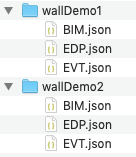
\includegraphics[width=0.2\textwidth]
    {figures/SWIM_demos.png} }
  \caption{Experiment files}
  \label{fig:demos}
\end{figure}

When an experiment data is loaded successfully, the ``Wall info" tab will show up \Cref{fig:bim}.
Where the user can choose to display the information of each floor, view the geometry, the material being used, and the layout of the reinforcement bars.
No edit is allowed in this tab, because this shall be the description of the experiment which is a fact.

\begin{figure}[!htbp]
  \centering {
    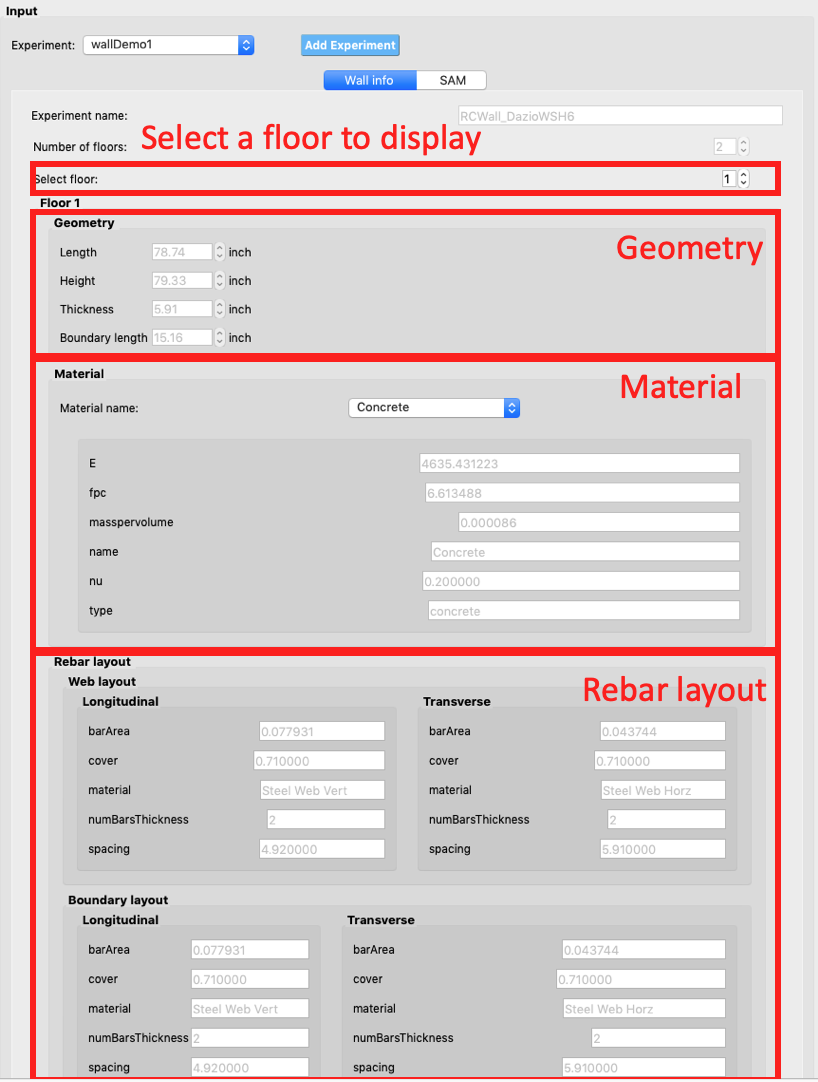
\includegraphics[width=0.8\textwidth]
    {figures/SWIM_input.png} }
  \caption{The ``Wall info" tab}
  \label{fig:bim}
\end{figure}

While the experiment being loaded, the application will automatically process the data and pick up suitable material models to show in the ``SAM" tab.
Meanwhile, the geometry of the wall will be displayed on the right of the application.
Inside the ``SAM" tab, the users can edit to control the mesh density and the parameters of the material model \Cref{fig:sam}. 


\begin{figure}[!htbp]
  \centering {
    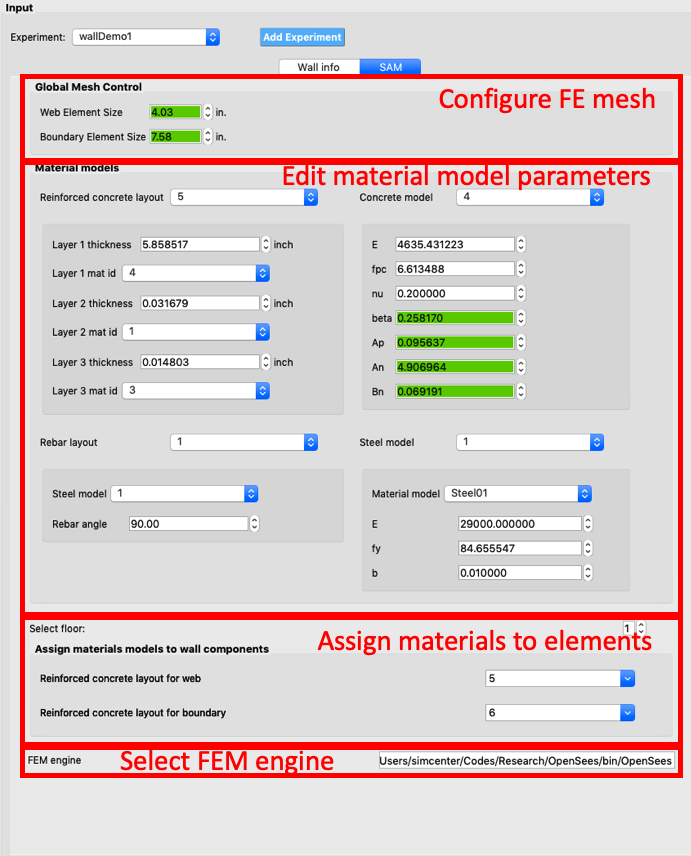
\includegraphics[width=0.8\textwidth]
    {figures/SWIM_SAM.png} }
  \caption{The ``SAM" tab}
  \label{fig:sam}
\end{figure}




In the ``Global Mesh Control" section inside the SAM tab, users can specify the element size of the finite element mesh. 
By default, the mesh sizes are set to be maximum values, so that the user can see the geometry of the wall rendered in grey color in the ``Shape" section on the right  \Cref{fig:shape} (a). 
When the use edit the sizes, the geometry will be replaced with element mesh rendered in blue \Cref{fig:shape} (b). 
If the user click the AI button at the bottom of the Input panel, the geometry will be replaced by green colored elements generated by AI \Cref{fig:shape} (c).

\begin{figure}[!htbp]
  \centering 
  \subfloat[Wall geometry]{
    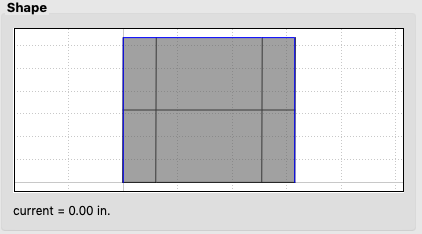
\includegraphics[width=0.39\textwidth]
    {figures/SWIM_shape_1.png}}
  \subfloat[User specified mesh]{
    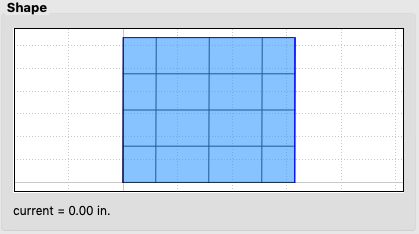
\includegraphics[width=0.39\textwidth]
    {figures/SWIM_shape_2.png}}
    
    \subfloat[Mesh generated by AI]{
    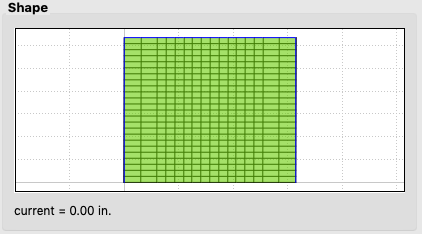
\includegraphics[width=0.39\textwidth]
    {figures/SWIM_shape_3.png}}
  \caption{Shape and mesh visualization}
  \label{fig:shape}
\end{figure}


While the AI button being clicked, several parameters will be edited by AI, including:
\begin{enumerate}
\item Web Element Size
\item Boundary Element Size
\item beta (Concrete model)
\item Ap (Concrete model)
\item An (Concrete model)
\item Bn (concrete model)
\end{enumerate}
Their color will be changed to green indicating these are AI predicted values \Cref{fig:colors}.
When the user try to edit these values, their color will be returned to white, 
while the mesh color being returned to blue \Cref{fig:shape} (b), 
indicating these settings are set by the user.

\begin{figure}[!htbp]
  \centering 
  \subfloat[Default settings]{
    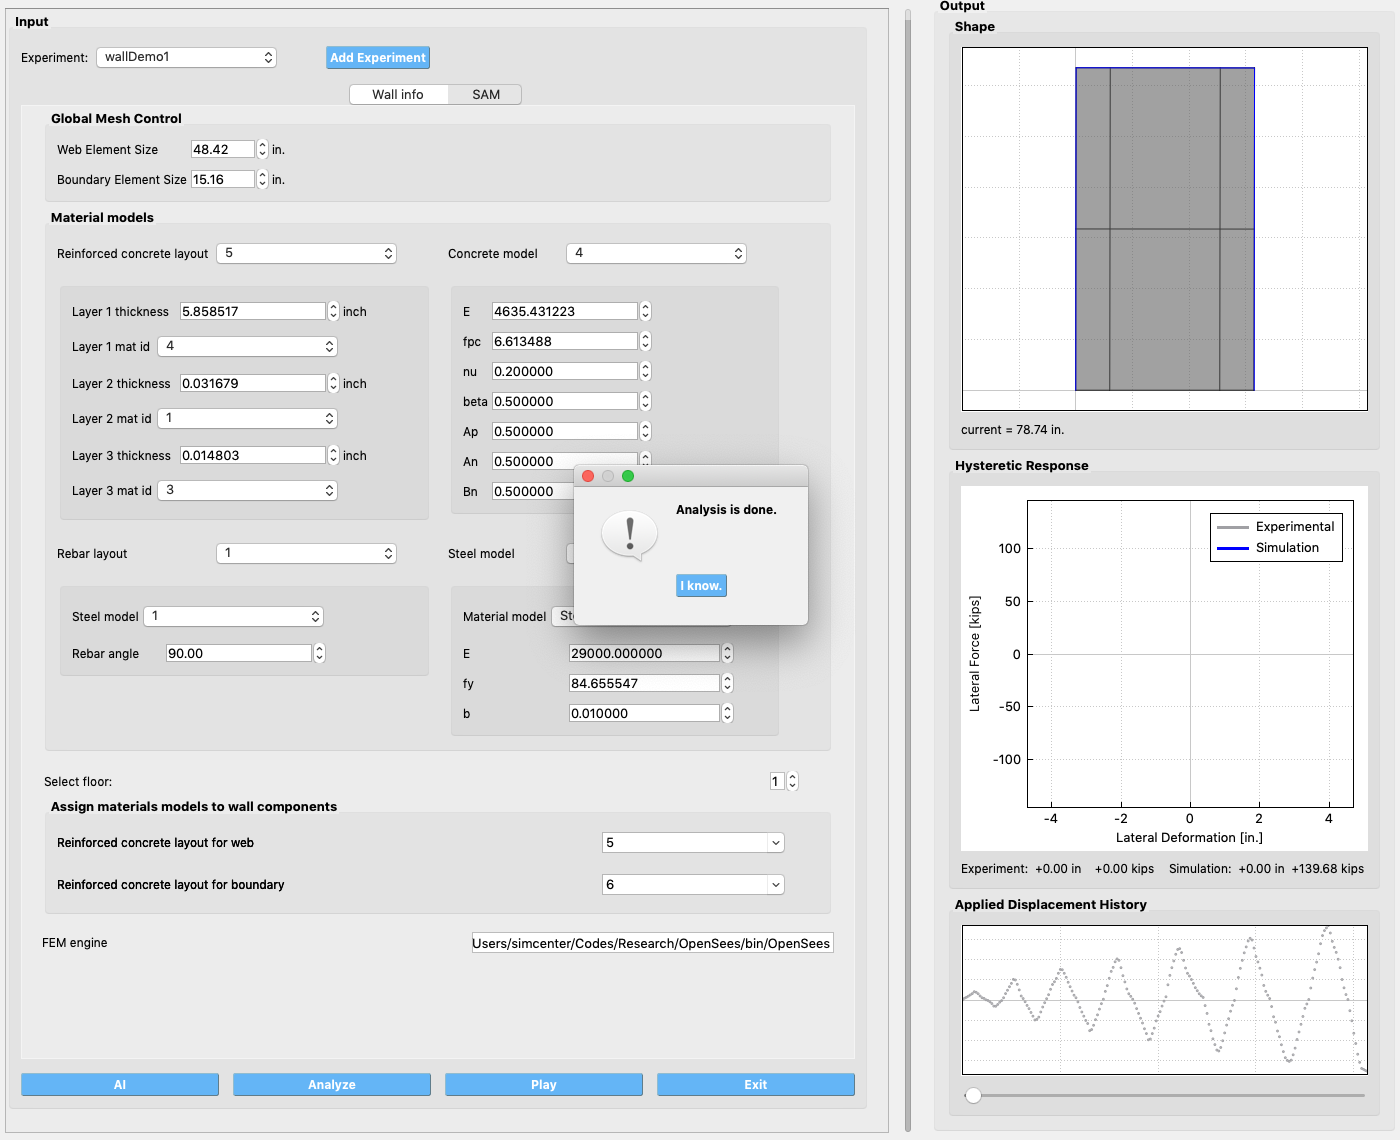
\includegraphics[width=0.47\textwidth]
    {figures/SWIM_grey.png}}
  \subfloat[AI settings, colored in green]{
    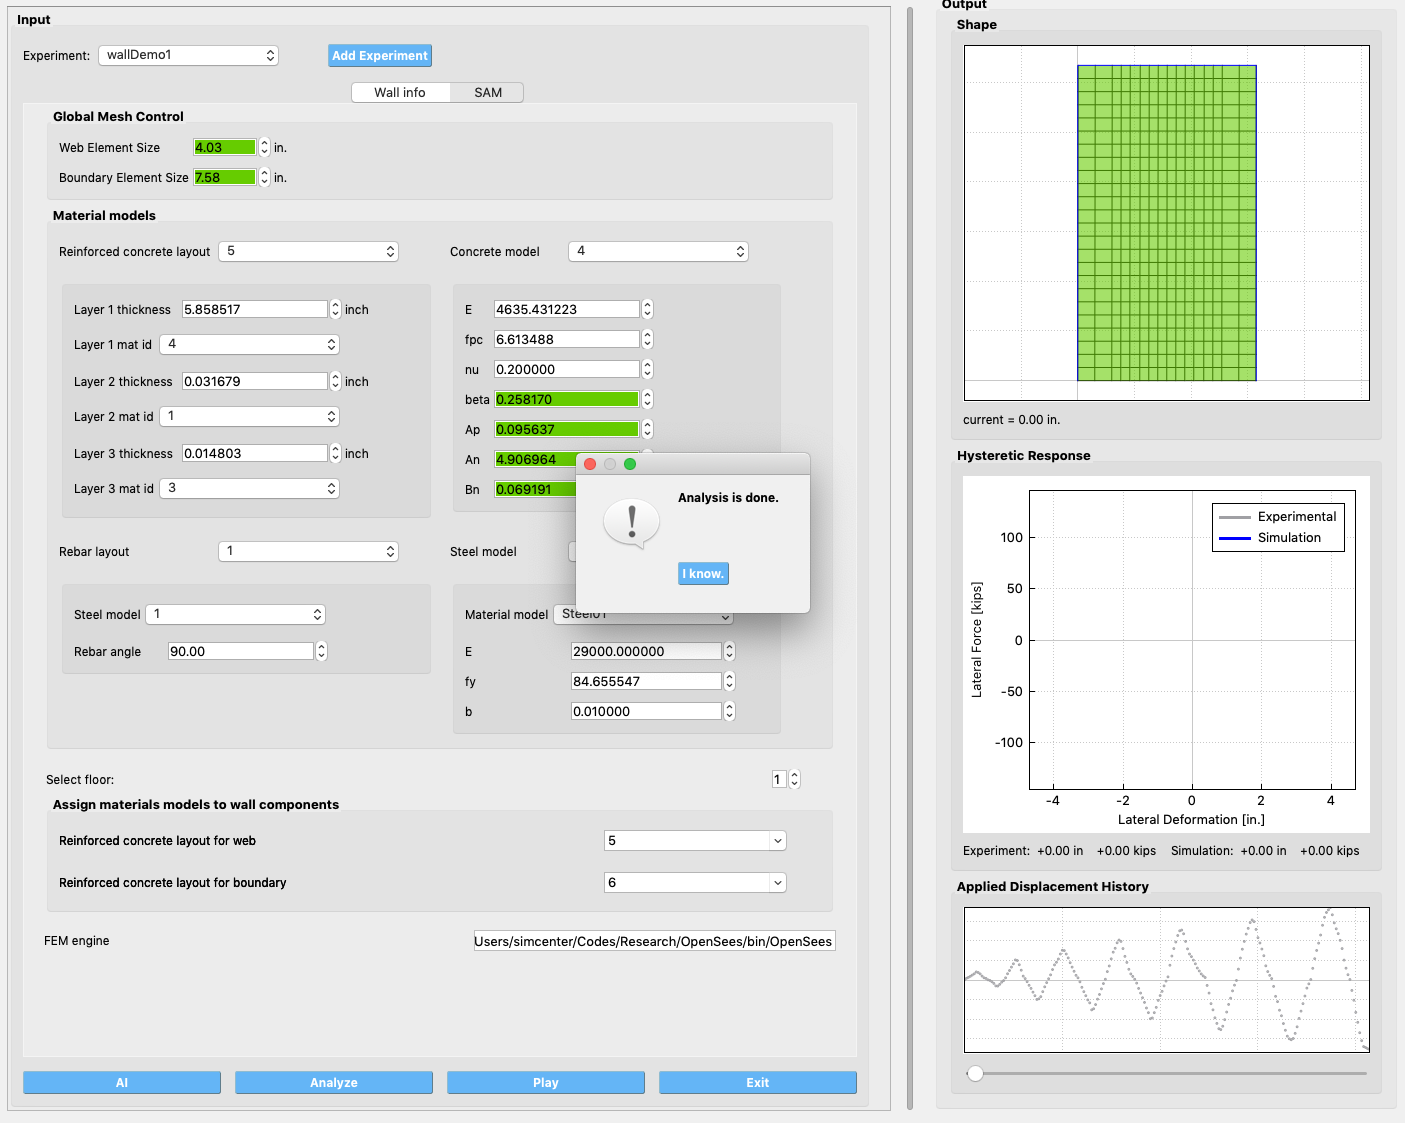
\includegraphics[width=0.48\textwidth]
    {figures/SWIM_green.png}}

  \caption{Call AI}
  \label{fig:colors}
\end{figure}

At the bottom of the SAM tab, the user need to provide the path of a finite element program. 
This version only support OpenSees. 

Once the users finished the editing, they can click ``Analyze" button. 
This will bring up a progress bar shown between the Input and Output panels.
When the analysis is completed, a message windows will pop up. The user can click ``I know.", then click ``Play'' button.
The animations will start in the Output panel, including:
the deformed mesh, the hysteretic curves and the load history. 

\begin{figure}[!htbp]
  \centering {
    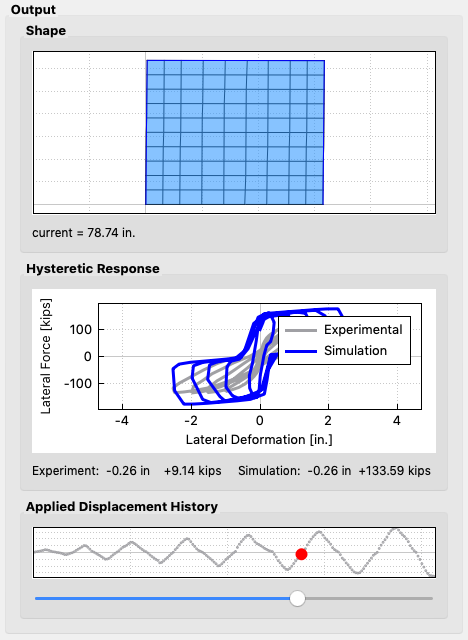
\includegraphics[width=0.8\textwidth]
    {figures/SWIM_output.png} }
  \caption{ Output tab}
  \label{fig:output}
\end{figure}

%Select a soil layer by clicking on the design table or by clicking on the graphic soil column.
%When a layer is selected, it will be highlighted in both the design table and the graphic. 
%In the design table, it is highlighted by changing the background color to light green. 


%Given that the properties of the soil layers and the earthquake events are known,
 %\texttt{\getsoftwarename{}} convert provide multiple nonlinear material models for simulating the soil behavior under earthquake loading.


\chapter{Theory and Implementation}
\label{chap:theory}
In the proposed model, planar quadrilateral elements adopting bilinear isoparametric representation of element geometry and shape functions \cite{bathe1976numerical} are coupled with the layered-section model proposed by \cite{lu2015shear}.

A plane-stress concrete material model which was developed based on the three-dimensional model proposed by \cite{faria1998strain}. The formulation is based on continuum damage mechanics and defines a relation between the response in a non-damaged effective space and a damaged physical space through an increasing damage variable. In addition to parameters based on material properties (such as Young modulus, Poisson ration, yield strength, etc.), representation of the material in-plane constitutive behavior is obtained through other four independent parameters: a coefficient $\beta$  governing the plastic strain rate and three damage parameters governing the damage evolution: Ap, An, Bn.



\begin{figure}[!htbp]
  \centering {
    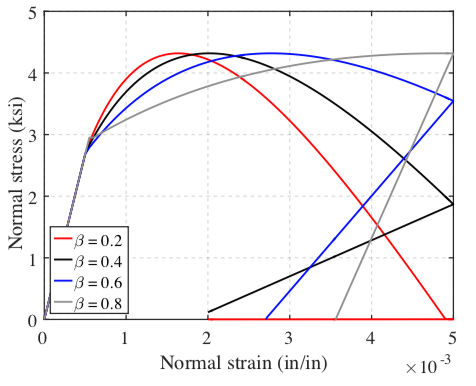
\includegraphics[width=0.7\textwidth]
    {figures/SWIM_beta.png} }
  \caption{ Effect of $\beta$ on the stress-strain relation and damage evolution}
  \label{fig:beta}
\end{figure}

An appropriate selection of the parameters that define the cyclic behavior of concrete is fundamental to capturing the response of RC shear walls at both the global and local level.

Plastic strain rate coefficient, $\beta$ governs the post-yield hardening modulus in the effective (undamaged) space and the plastic strain rate. 
\Cref{fig:beta} shows sample stress-strain relation with complete load removal at strain value of $5x10^{-3}$ to illustrate the effect of $\beta$. 
A higher value of $\beta$ increases the amount of plastic strain accumulated. 
A special case of $\beta$ = 0 represents elastic behavior with elastic unloading. 
Typical values of $\beta$ are 0.3 - 0.6.


\begin{figure}[!htbp]
  \centering {
    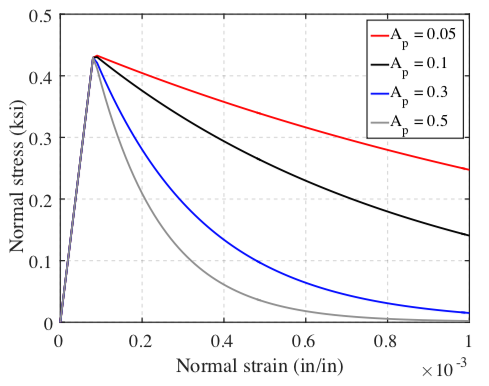
\includegraphics[width=0.7\textwidth]
    {figures/SWIM_Ap.png} }
  \caption{ Effect of Ap on the stress-strain relation}
  \label{fig:Ap}
\end{figure}

Parameter Ap governs the tensile fracture energy and affects the ”ductility” of the tensile response. Fig. 2 shows the effect of parameter Ap on the response in uniaxial tension for different values of Ap. A higher Ap results in a more ductile tensile response. \cite{faria1998strain} suggests an expression to relate Ap to the characteristic length $l_{ch}$ and fracture energy $G_f$:

\begin{equation}
A_p=\left(\frac{G_fE}{l_{ch}(f_t)^2}-\frac{1}{2}\right)^{-1}\geq 0
\end{equation}




\begin{figure}[!htbp]
  \centering {
    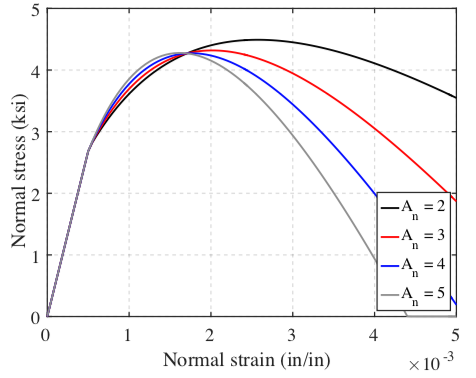
\includegraphics[width=0.7\textwidth]
    {figures/SWIM_An.png} }
  \caption{ Effect of An on the stress-strain relation}
  \label{fig:An}
\end{figure}

\begin{figure}[!htbp]
  \centering {
    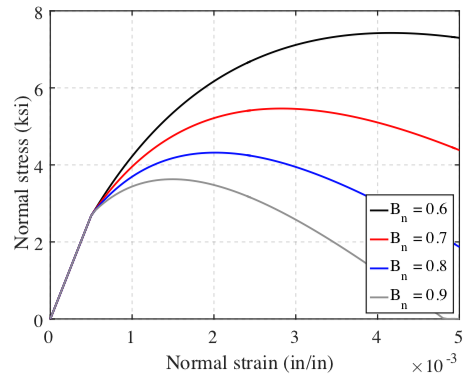
\includegraphics[width=0.7\textwidth]
    {figures/SWIM_Bn.png} }
  \caption{ Effect of Bn on the stress-strain relation}
  \label{fig:Bn}
\end{figure}

Parameters An and Bn govern the softening behavior of concrete in compression. \Cref{fig:An} and \Cref{fig:Bn} show the effect of parameters An and Bn on the response of uniaxial compression for different values of the parameters. 
Both parameters affect the ductility of the compressive response; 
however, parameter An changes the ductility but does not alter the peak strength significantly, 
whereas parameter Bn changes both the ductility and the peak strength. 
It is noteworthy that the numerical solution is rather sensitive to change in parameter Bn.



For modeling reinforcing steel, any uniaxial steel material constitutive model can be used provided it is embedded in the plane stress material object, whereby the steel is assigned a direction and a plane stress tensor is constructed.







\chapter{Source Code}
\label{chap:SourceCode}
This source code for the tool is released under the 2-clause BSD
License, commonly called the FreeBSD license.  It is available for
download from the
tool's \href{https://github.com/NHERI-SimCenter/SWIM}{GitHub
repository}.

\chapter{User Training}
\label{chap:training}
User Training consists of an online video available from the tool
webpage that demonstrates tool use. The tool will be presented in user
workshops hosted by the SimCenter.



\chapter{Verification and Validation by Examples}
\label{chap:vnv}
\subsection{Squat wall}

The concrete shear wall being tested in this example is WhittakerSW5 which is 39.6 inches tall (one-story) and 120 inches wide. 
The specimen was tested under cyclic-static action. 
In SWIM, the wall is simulated using 4-node quad plane stress elements. 
Nodes at the bottom are fixed and cyclic displacements are applied to nodes at the top. 
Self weight is distributed to each node as vertical load.
The simulated results are compared with the experiment in \Cref{fig:WhittSW5}.



\begin{figure}[!htbp]
  \centering {
    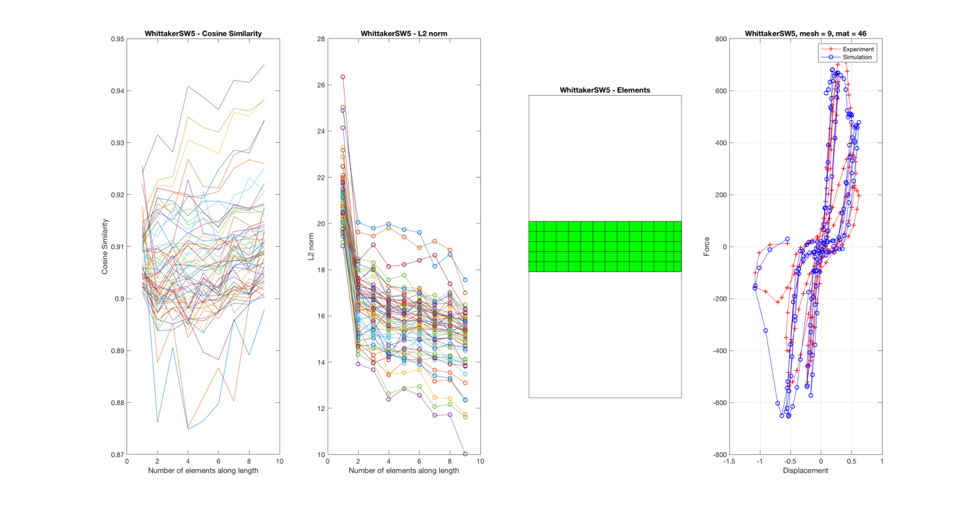
\includegraphics[width=0.95\textwidth]
    {figures/SWIM_WhittSW5.png} }
  \caption{WhittakerSW5}
  \label{fig:WhittSW5}
\end{figure}




\subsection{Tall wall}

The concrete shear wall being tested in this example is OesterleB3 which is 176 inches tall (4 stories) and 75 inches wide. 
The specimen was tested under cyclic-static action. 
In SWIM, the wall is simulated using 4-node quad plane stress elements. 
Nodes at the bottom are fixed and cyclic displacements are applied to nodes at the top. 
Self weight is distributed to each node as vertical load.
The simulated results are compared with the experiment in \Cref{fig:OesterleB3}.


\begin{figure}[!htbp]
  \centering {
    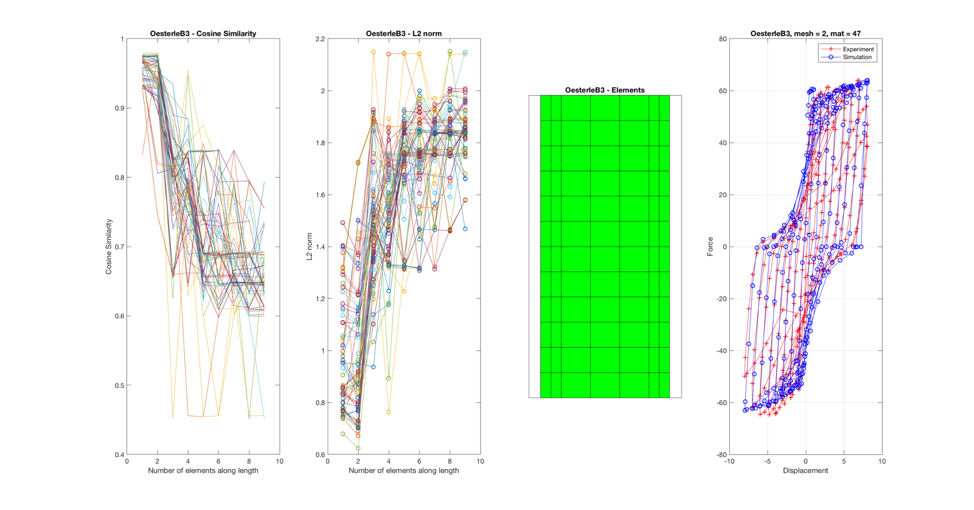
\includegraphics[width=0.95\textwidth]
    {figures/SWIM_OB3.png} }
  \caption{OesterleB3}
  \label{fig:OesterleB3}
\end{figure}





\nocite{*}

% \appendix
% \chapter{More Monticello Candidates}

\pagestyle{plain}
{
  \renewcommand{\thispagestyle}[1]{}	
  \printbibliography           
}

\end{document}
